\section{Мета роботи}
Закріпити теоретичні знання та набути практичного досвіду
впорядкування набору статичних та динамічних структур даних.

\section{Хід роботи}
Написати програму, що реалізує три алгоритми сортування набору
даних згідно з табл. 12.1.\\

Визначити кількість порівнянь та обмінів для початкових наборів
даних, що містять різну кількість елементів (50, 1000, 5000, 10000, 50000).\\

Оцінити час сортування. Дослідити вплив початкової впорядкованості
набору даних (відсортований, відсортований у зворотному порядку,
випадковий).\\

Всі отримані дані записати в табл. 12.2. Зробити висновки.\\

\textbf{Моє завдання:} \\
Алгоритми сортування:
\begin{itemize}
  \item сортування частково впорядкованим деревом
  \item порозрядне цифрове сортування
  \item сортування прямим злиттям
\end{itemize}
Массив: своя структура динамічного массиву\\

\clearpage
\subsection{Реалізація динамічного масиву}
У структурі було створено методи: \textit{ініціалізації, знищення, додавання елементів, отримання елементів}.\\

Файл \textbf{заголовків}
\begin{lstlisting}[style=customc]
#ifndef DYN_ARR_H
#define DYN_ARR_H

#include <stdio.h>
#include <stdlib.h>

typedef struct DynArr
{
  void *data;
  size_t elem_size;
  size_t size;
  size_t capacity;
} DynArr;

DynArr *init_dyn_arr(size_t element_size, size_t initial_capacity);
void push_dyn_arr(DynArr *array, void *element);
void *get_elem_dyn_arr(DynArr *array, size_t index);
void destroy_dyn_arr(DynArr *array);

#endif
\end{lstlisting}

Файл \textbf{реалізації}
\begin{lstlisting}[style=customc]
#include "dyn_arr.h"

// init arr
DynArr *init_dyn_arr(size_t element_size, size_t initial_capacity)
{
  DynArr *arr = malloc(sizeof(DynArr));
  if (!arr)
  {
    perror("Failed to allocate memory for array");
    exit(EXIT_FAILURE);
  }

  arr->data = calloc(element_size, initial_capacity);
  if (!arr->data)
  {
    perror("Failed to allocate memory for array data");
    free(arr);
    exit(EXIT_FAILURE);
  }

  arr->elem_size = element_size;
  arr->size = 0;
  arr->capacity = initial_capacity;

  return arr;
}

// resize arr
void _resize_arr(DynArr *arr, size_t new_capacity)
{
  arr->data = realloc(arr->data, arr->elem_size * new_capacity);
  if (!arr->data)
  {
    perror("Failed to reallocate memory");
    exit(EXIT_FAILURE);
  }
  arr->capacity = new_capacity;
}

// push elem to arr
void push_dyn_arr(DynArr *arr, void *element)
{
  if (arr->size == arr->capacity)
  {
    _resize_arr(arr, arr->capacity * 2);
  }

  memcpy((char *)arr->data + arr->size * arr->elem_size, element, arr->elem_size);
  arr->size++;
}

// get elem by index from arr
void *get_elem_dyn_arr(DynArr *arr, size_t index)
{
  if (index >= arr->size)
  {
    fprintf(stderr, "Index out of bounds\n");
    return NULL;
  }
  return (char *)arr->data + index * arr->elem_size;
}

// destroy arr
void destroy_dyn_arr(DynArr *arr)
{
  free(arr->data);
  free(arr);
}
\end{lstlisting}

\clearpage
\subsection{Реалізація сортувань}
Всі сортування було створено та об`єднано спеціальною структурою для того щоб виводити однакові метрики для всі сортувань. Кожна функція приймає структуру динамічного масиву та порядок сортування та виведе на екран кількість перестановок та порівнянь. Окрім сортування частоково впорядкованими деревами, яке ще приймає функцію порівняння.

\subsubsection{Реалізація алгоритму сортування злиттям}
\begin{lstlisting}[style=customc]
  #include "merge_sort.h"

  int compare_elements(void *a, void *b, size_t elem_size, SortOrder order)
  {
    if (order == ASCENDING)
    {
      return memcmp(a, b, elem_size);
    }
    else
    {
      return memcmp(b, a, elem_size);
    }
  }
  
  void merge(DynArr *arr, size_t left, size_t mid, size_t right, SortOrder order, SortStats *stats)
  {
    size_t left_size = mid - left + 1;
    size_t right_size = right - mid;
  
    void *left_arr = malloc(left_size * arr->elem_size);
    void *right_arr = malloc(right_size * arr->elem_size);
  
    if (!left_arr || !right_arr)
    {
      perror("Failed to allocate memory for merge");
      exit(EXIT_FAILURE);
    }
  
    memcpy(left_arr, (char *)arr->data + left * arr->elem_size, left_size * arr->elem_size);
    memcpy(right_arr, (char *)arr->data + (mid + 1) * arr->elem_size, right_size * arr->elem_size);
  
    size_t i = 0, j = 0, k = left;
  
    while (i < left_size && j < right_size)
    {
      stats->comparisons++;
      if (compare_elements((char *)left_arr + i * arr->elem_size, (char *)right_arr + j * arr->elem_size, arr->elem_size, order) <= 0)
      {
        memcpy((char *)arr->data + k * arr->elem_size, (char *)left_arr + i * arr->elem_size, arr->elem_size);
        i++;
      }
      else
      {
        memcpy((char *)arr->data + k * arr->elem_size, (char *)right_arr + j * arr->elem_size, arr->elem_size);
        j++;
      }
      k++;
      stats->swaps++;
    }
  
    while (i < left_size)
    {
      memcpy((char *)arr->data + k * arr->elem_size, (char *)left_arr + i * arr->elem_size, arr->elem_size);
      i++;
      k++;
      stats->swaps++;
    }
  
    while (j < right_size)
    {
      memcpy((char *)arr->data + k * arr->elem_size, (char *)right_arr + j * arr->elem_size, arr->elem_size);
      j++;
      k++;
      stats->swaps++;
    }
  
    free(left_arr);
    free(right_arr);
  }
  
  void merge_sort(DynArr *arr, size_t left, size_t right, SortOrder order, SortStats *stats)
  {
    if (left < right)
    {
      size_t mid = left + (right - left) / 2;
  
      merge_sort(arr, left, mid, order, stats);
      merge_sort(arr, mid + 1, right, order, stats);
      merge(arr, left, mid, right, order, stats);
    }
  }
  
  void merge_sort_dyn_arr(DynArr *arr, SortOrder order)
  {
    SortStats stats = {0, 0};
    merge_sort(arr, 0, arr->size - 1, order, &stats);
  
    if (order == ASCENDING)
    {
      printf("\n\033[32m\033[0m Sorting order: \033[32masc\033[0m\n");
    }
    else
    {
      printf("\n\033[32m\033[0m Sorting order: \033[32mdesc\033[0m\n");
    }
  
    printf("\033[32m󰓡\033[0m Number of swaps: \033[32m%d\033[0m\n", stats.swaps);
    printf("\033[32m\033[0m Number of comparisons: \033[32m%d\033[0m\n", stats.comparisons);
  }
\end{lstlisting}

\subsubsection{Реалізація алгоритму порозрядного цифрового сортування}
\begin{lstlisting}[style=customc]
#include "radix_sort.h"

int get_digit(int number, int place)
{
  return (number / place) % 10;
}

int get_max(DynArr *arr)
{
  int max = *(int *)get_elem_dyn_arr(arr, 0);
  for (size_t i = 1; i < arr->size; i++)
  {
    int value = *(int *)get_elem_dyn_arr(arr, i);
    if (value > max)
    {
      max = value;
    }
  }
  return max;
}

void counting_sort(DynArr *arr, int place, SortOrder order, SortStats *stats)
{
  size_t count[10] = {0};
  int *output = malloc(arr->size * sizeof(int));

  if (!output)
  {
    perror("Failed to allocate memory for output array");
    exit(EXIT_FAILURE);
  }

  for (size_t i = 0; i < arr->size; i++)
  {
    int digit = get_digit(*(int *)get_elem_dyn_arr(arr, i), place);
    count[digit]++;
  }

  if (order == ASCENDING)
  {
    for (int i = 1; i < 10; i++)
    {
      count[i] += count[i - 1];
    }
  }
  else
  {
    for (int i = 8; i >= 0; i--)
    {
      count[i] += count[i + 1];
    }
  }

  for (int i = arr->size - 1; i >= 0; i--)
  {
    int digit = get_digit(*(int *)get_elem_dyn_arr(arr, i), place);
    output[--count[digit]] = *(int *)get_elem_dyn_arr(arr, i);
    stats->swaps++;
  }

  for (size_t i = 0; i < arr->size; i++)
  {
    memcpy((char *)arr->data + i * arr->elem_size, &output[i], sizeof(int));
  }

  free(output);
}

void radix_sort(DynArr *arr, SortOrder order, SortStats *stats)
{
  int max = get_max(arr);

  for (int place = 1; max / place > 0; place *= 10)
  {
    counting_sort(arr, place, order, stats);
    stats->comparisons += arr->size;
  }
}

void radix_sort_dyn_arr(DynArr *arr, SortOrder order)
{
  SortStats stats = {0, 0};
  radix_sort(arr, order, &stats);

  if (order == ASCENDING)
  {
    printf("\n\033[32m\033[0m Sorting order: \033[32masc\033[0m\n");
  }
  else
  {
    printf("\n\033[32m\033[0m Sorting order: \033[32mdesc\033[0m\n");
  }

  printf("\033[32m󰓡\033[0m Number of swaps: \033[32m%d\033[0m\n", stats.swaps);
  printf("\033[32m\033[0m Number of comparisons: \033[32m%d\033[0m\n", stats.comparisons);
}
\end{lstlisting}

\clearpage
\subsubsection{Реалізація алгоритму сортування частково впорядкованим деревом}
\begin{lstlisting}[style=customc]
#include <stdio.h>
#include <stdlib.h>
#include <string.h>
#include "heap_sort.h"

// Допоміжна функція для обміну двох елементів масиву
static void swap_elements(DynArr *arr, size_t i, size_t j, SortStats *stats)
{
  if (i == j)
    return;
  // Виділяємо тимчасовий буфер під один елемент
  void *temp = malloc(arr->elem_size);
  if (!temp)
  {
    perror("Failed to allocate memory for swap");
    exit(EXIT_FAILURE);
  }

  void *elem_i = (char *)arr->data + i * arr->elem_size;
  void *elem_j = (char *)arr->data + j * arr->elem_size;

  memcpy(temp, elem_i, arr->elem_size);
  memcpy(elem_i, elem_j, arr->elem_size);
  memcpy(elem_j, temp, arr->elem_size);

  free(temp);

  stats->swaps++;
}

// Допоміжна функція для порівняння елементів та підрахунку порівнянь
static int compare_elements(const void *a, const void *b, int (*compare)(const void *, const void *), SortStats *stats)
{
  stats->comparisons++;
  return compare(a, b);
}

// Підтримка властивостей купи (heapify)
// Для сортування за зростанням - будуємо max-heap (батько більший за нащадків).
// Для сортування за спаданням - будуємо min-heap (батько менший за нащадків).
static void heapify(DynArr *arr, size_t n, size_t i, SortOrder order, int (*compare)(const void *, const void *), SortStats *stats)
{
  size_t largest_or_smallest = i;
  size_t left = 2 * i + 1;
  size_t right = 2 * i + 2;

  // Залежно від порядку, вибираємо напрямок порівняння
  // Для ASCENDING: ми хочемо max-heap, тобто батько має бути більшим за дітей.
  // largest_or_smallest буде найбільшим
  // Для DESCENDING: ми хочемо min-heap, тобто батько має бути меншим за дітей.
  // largest_or_smallest буде найменшим.

  // Перевірка лівого нащадка
  if (left < n)
  {
    void *current = (char *)arr->data + largest_or_smallest * arr->elem_size;
    void *child = (char *)arr->data + left * arr->elem_size;
    int cmp = compare_elements(child, current, compare, stats);

    if ((order == ASCENDING && cmp > 0) || (order == DESCENDING && cmp < 0))
    {
      largest_or_smallest = left;
    }
  }

  // Перевірка правого нащадка
  if (right < n)
  {
    void *current = (char *)arr->data + largest_or_smallest * arr->elem_size;
    void *child = (char *)arr->data + right * arr->elem_size;
    int cmp = compare_elements(child, current, compare, stats);

    if ((order == ASCENDING && cmp > 0) || (order == DESCENDING && cmp < 0))
    {
      largest_or_smallest = right;
    }
  }

  // Якщо найбільший/найменший не батько, то міняємо місцями та продовжуємо
  if (largest_or_smallest != i)
  {
    swap_elements(arr, i, largest_or_smallest, stats);
    heapify(arr, n, largest_or_smallest, order, compare, stats);
  }
}

void heap_sort_dyn_arr(DynArr *arr, SortOrder order, int (*compare)(const void *, const void *))
{
  SortStats stats = {0, 0};

  size_t n = arr->size;
  if (n < 2)
  {
    // Масив уже відсортований або недостатньо даних для сортування
    if (order == ASCENDING)
    {
      printf("\n\033[32m\033[0m Sorting order: \033[32masc\033[0m\n");
    }
    else
    {
      printf("\n\033[32m\033[0m Sorting order: \033[32mdesc\033[0m\n");
    }

    printf("\033[32m󰓡\033[0m Number of swaps: \033[32m%zu\033[0m\n", stats.swaps);
    printf("\033[32m\033[0m Number of comparisons: \033[32m%zu\033[0m\n", stats.comparisons);
    return;
  }

  // Побудова купи
  for (int i = (int)(n / 2) - 1; i >= 0; i--)
  {
    heapify(arr, n, (size_t)i, order, compare, &stats);
  }

  // Послідовне "виймання" елементів з купи
  for (size_t i = n - 1; i > 0; i--)
  {
    swap_elements(arr, 0, i, &stats);
    heapify(arr, i, 0, order, compare, &stats);
  }

  if (order == ASCENDING)
  {
    printf("\n\033[32m\033[0m Sorting order: \033[32masc\033[0m\n");
  }
  else
  {
    printf("\n\033[32m\033[0m Sorting order: \033[32mdesc\033[0m\n");
  }

  printf("\033[32m󰓡\033[0m Number of swaps: \033[32m%zu\033[0m\n", stats.swaps);
  printf("\033[32m\033[0m Number of comparisons: \033[32m%zu\033[0m\n", stats.comparisons);
}
\end{lstlisting}

\clearpage
\subsubsection{Реалізація програми лабораторної роботи}
У програмі створюється динамічний масив та заповнюється випалковими цілими числами. Також додатково реалізовані функції рахування часу виконання алгоритму та виводу масиву у консоль у приємному вигляді.
\begin{lstlisting}[style=customc]
#include <stdio.h>
#include <stdlib.h>

#include "general_utils.h"

#include "heap_sort.h"
#include "radix_sort.h"
#include "merge_sort.h"

#include "time.h"

int int_compare(const void *a, const void *b)
{
  int x = *(const int *)a;
  int y = *(const int *)b;
  return (x - y);
}

void print_array(DynArr *arr)
{
  for (int i = 0; i < arr->size; i++)
  {
    int *value = (int *)get_elem_dyn_arr(arr, i);
    if (i == 0)
    {
      printf("[ %d ", *value);
    }
    else if (i == arr->size - 1)
    {
      printf(" %d ]", *value);
    }
    else
    {
      printf(" %d ", *value);
    }
  }

  printf("\nArray size: %zu\n", arr->size);
}

void generate_arr_data(DynArr *arr)
{
  for (int i = 0; i < arr->capacity; i++)
  {
    int value = generateRandomInt(1, 99);
    push_dyn_arr(arr, &value);
  }
}

void measure_execution_time_for_heap(int (*func)(DynArr *arr, SortOrder *order, int (*compare)(const void *, const void *)), const DynArr *arr, SortOrder *order, int (*compare)(const void *, const void *))
{
  clock_t start = clock();
  func(arr, order, compare);
  clock_t end = clock();

  double time_taken_ms = ((double)(end - start)) / CLOCKS_PER_SEC * 1000;
  printf("\033[32m\033[0m Estimated time: \033[32m%.2f\033[0m ms\n", time_taken_ms);
}

void measure_execution_time(int (*func)(DynArr *arr, SortOrder *order), const DynArr *arr, SortOrder *order)
{
  clock_t start = clock();
  func(arr, order);
  clock_t end = clock();

  double time_taken_ms = ((double)(end - start)) / CLOCKS_PER_SEC * 1000;
  printf("\033[32m\033[0m Estimated time: \033[32m%.2f\033[0m ms\n", time_taken_ms);
}

void task1()
{
  srand(time(NULL));

  int ARR_SIZE = 50;
  DynArr *int_arr = init_dyn_arr(sizeof(int), ARR_SIZE);

  generate_arr_data(int_arr);

  highlightText("DYNAMIC ARRAY OF INT VALUES", "blue");
  print_array(int_arr);

  highlightText("\nDYNAMIC ARRAY OF INT VALUES AFTER HEAP SORT", "yellow");
  measure_execution_time_for_heap(heap_sort_dyn_arr, int_arr, ASCENDING, int_compare);

  highlightText("\nDYNAMIC ARRAY OF INT VALUES AFTER RADIX SORT", "yellow");
  measure_execution_time(radix_sort_dyn_arr, int_arr, ASCENDING);

  highlightText("\nDYNAMIC ARRAY OF INT VALUES AFTER MERGE SORT", "yellow");
  measure_execution_time(merge_sort_dyn_arr, int_arr, ASCENDING);

  print_array(int_arr);

  destroy_dyn_arr(int_arr);

  return 0;
}
\end{lstlisting}


\clearpage
\subsection{Результати роботи програми:}
\subsubsection{Тестування алгоритмів для масиву з 15 елементів}
\begin{figure}[h!]
  \centering
  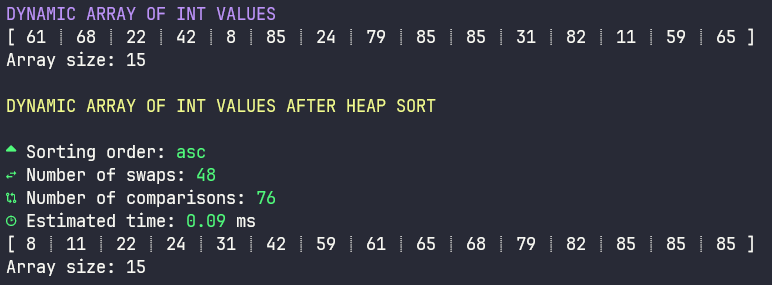
\includegraphics[width=15cm]{reports/algos/lab12/assets/heap.png}
  \caption{Результат сортування частково впорядкованим деревом}
\end{figure}

\begin{figure}[h!]
  \centering
  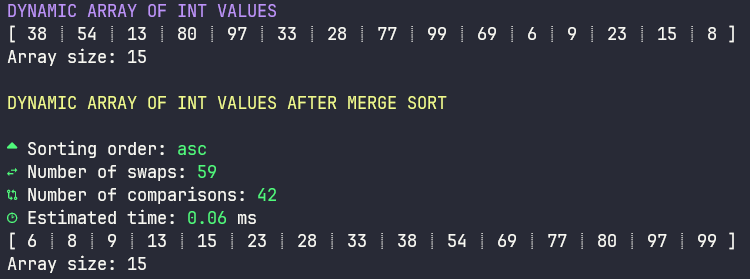
\includegraphics[width=15cm]{reports/algos/lab12/assets/merge.png}
  \caption{Результат сортування злиттям}
\end{figure}

\begin{figure}[h!]
  \centering
  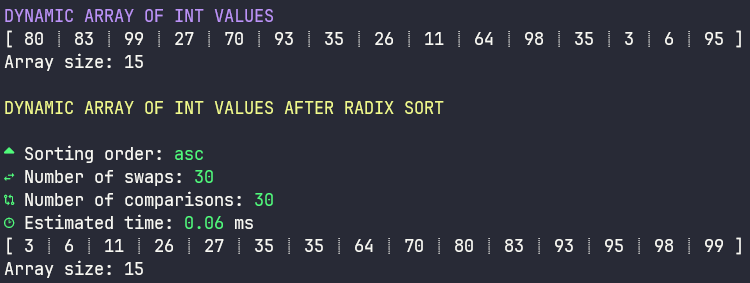
\includegraphics[width=15cm]{reports/algos/lab12/assets/radix.png}
  \caption{Результат порозрядного цифрового сортування}
\end{figure}

\clearpage
\subsubsection{Аналіз результатів сортування при різних розмірах масиву}

\begin{table}[htbp]
  \caption{Результати сортування злиттям}
  \resizebox{\textwidth}{!}{%
  \begin{tabular}{|l|c|c|c|c|c|}
  \hline
  \textit{\textbf{Відсортований набір даних}}          & \textbf{20} & \textbf{1000} & \textbf{5000} & \textbf{10000} & \textbf{50000} \\ \hline
  Кількість пересилань                                 & 88          & 9976          & 61808         & 133616         & 784464         \\ \hline
  Кількість порівнянь                                  & 66          & 8735          & 55153         & 120130         & 716680         \\ \hline
  Час сортування (мс.)                                 & 0.07        & 0.46          & 1.97          & 4.19           & 21.55          \\ \hline
  \textit{\textbf{Відсортований у зворотньму порядку}} & \textbf{20} & \textbf{1000} & \textbf{5000} & \textbf{10000} & \textbf{50000} \\ \hline
  Кількість пересилань                                 & 88          & 9976          & 61808         & 133616         & 784464         \\ \hline
  Кількість порівнянь                                  & 66          & 8691          & 55175         & 120235         & 716606         \\ \hline
  Час сортування (мс.)                                 & 0.07        & 0.44          & 2.27          & 4.40           & 20             \\ \hline
  \end{tabular}%
  }
\end{table}

\begin{table}[htbp]
  \caption{Результат порозрядного цифрового сортування}
  \resizebox{\textwidth}{!}{%
  \begin{tabular}{|l|c|c|c|c|c|}
  \hline
  \textit{\textbf{Відсортований набір даних (asc)}}           & \textbf{20} & \textbf{1000} & \textbf{5000} & \textbf{10000} & \textbf{50000} \\ \hline
  Кількість пересилань                                        & 40          & 2000          & 10000         & 20000          & 100000         \\ \hline
  Кількість порівнянь                                         & 40          & 2000          & 10000         & 20000          & 100000         \\ \hline
  Час сортування (мс.)                                        & 0.09        & 0.12          & 0.42          & 0.54           & 3.6            \\ \hline
  \textit{\textbf{Відсортований у зворотньму порядку (desc)}} & \textbf{20} & \textbf{1000} & \textbf{5000} & \textbf{10000} & \textbf{50000} \\ \hline
  Кількість пересилань                                        & 40          & 2000          & 10000         & 20000          & 100000         \\ \hline
  Кількість порівнянь                                         & 40          & 2000          & 10000         & 20000          & 100000         \\ \hline
  Час сортування (мс.)                                        & 0.05        & 0.12          & 0.3           & 0.74           & 3.6            \\ \hline
  \end{tabular}%
  }
\end{table}

\begin{table}[htbp]
  \caption{Результат сортування випадково впорядкованим деревом}
  \resizebox{\textwidth}{!}{%
  \begin{tabular}{|l|c|c|c|c|c|}
  \hline
  \textit{\textbf{Відсортований набір даних (asc)}}           & \textbf{20} & \textbf{1000} & \textbf{5000} & \textbf{10000} & \textbf{50000} \\ \hline
  Кількість пересилань                                        & 74          & 9002          & 56784         & 123327         & 731544         \\ \hline
  Кількість порівнянь                                         & 113         & 16804         & 107420        & 234426         & 1401449        \\ \hline
  Час сортування (мс.)                                        & 0.07        & 0.74          & 3.33          & 8.33           & 44.95          \\ \hline
  \textit{\textbf{Відсортований у зворотньму порядку (desc)}} & \textbf{20} & \textbf{1000} & \textbf{5000} & \textbf{10000} & \textbf{50000} \\ \hline
  Кількість пересилань                                        & 68          & 9007          & 56637         & 123308         & 731255         \\ \hline
  Кількість порівнянь                                         & 115         & 16791         & 107248        & 234358         & 1401659        \\ \hline
  Час сортування (мс.)                                        & 0.04        & 0.72          & 4.28          & 8.10           & 42.68          \\ \hline
  \end{tabular}%
  }
\end{table}


\clearpage
Графіки побудовані на основі таблиць:
\begin{figure}[h!]
  \centering
  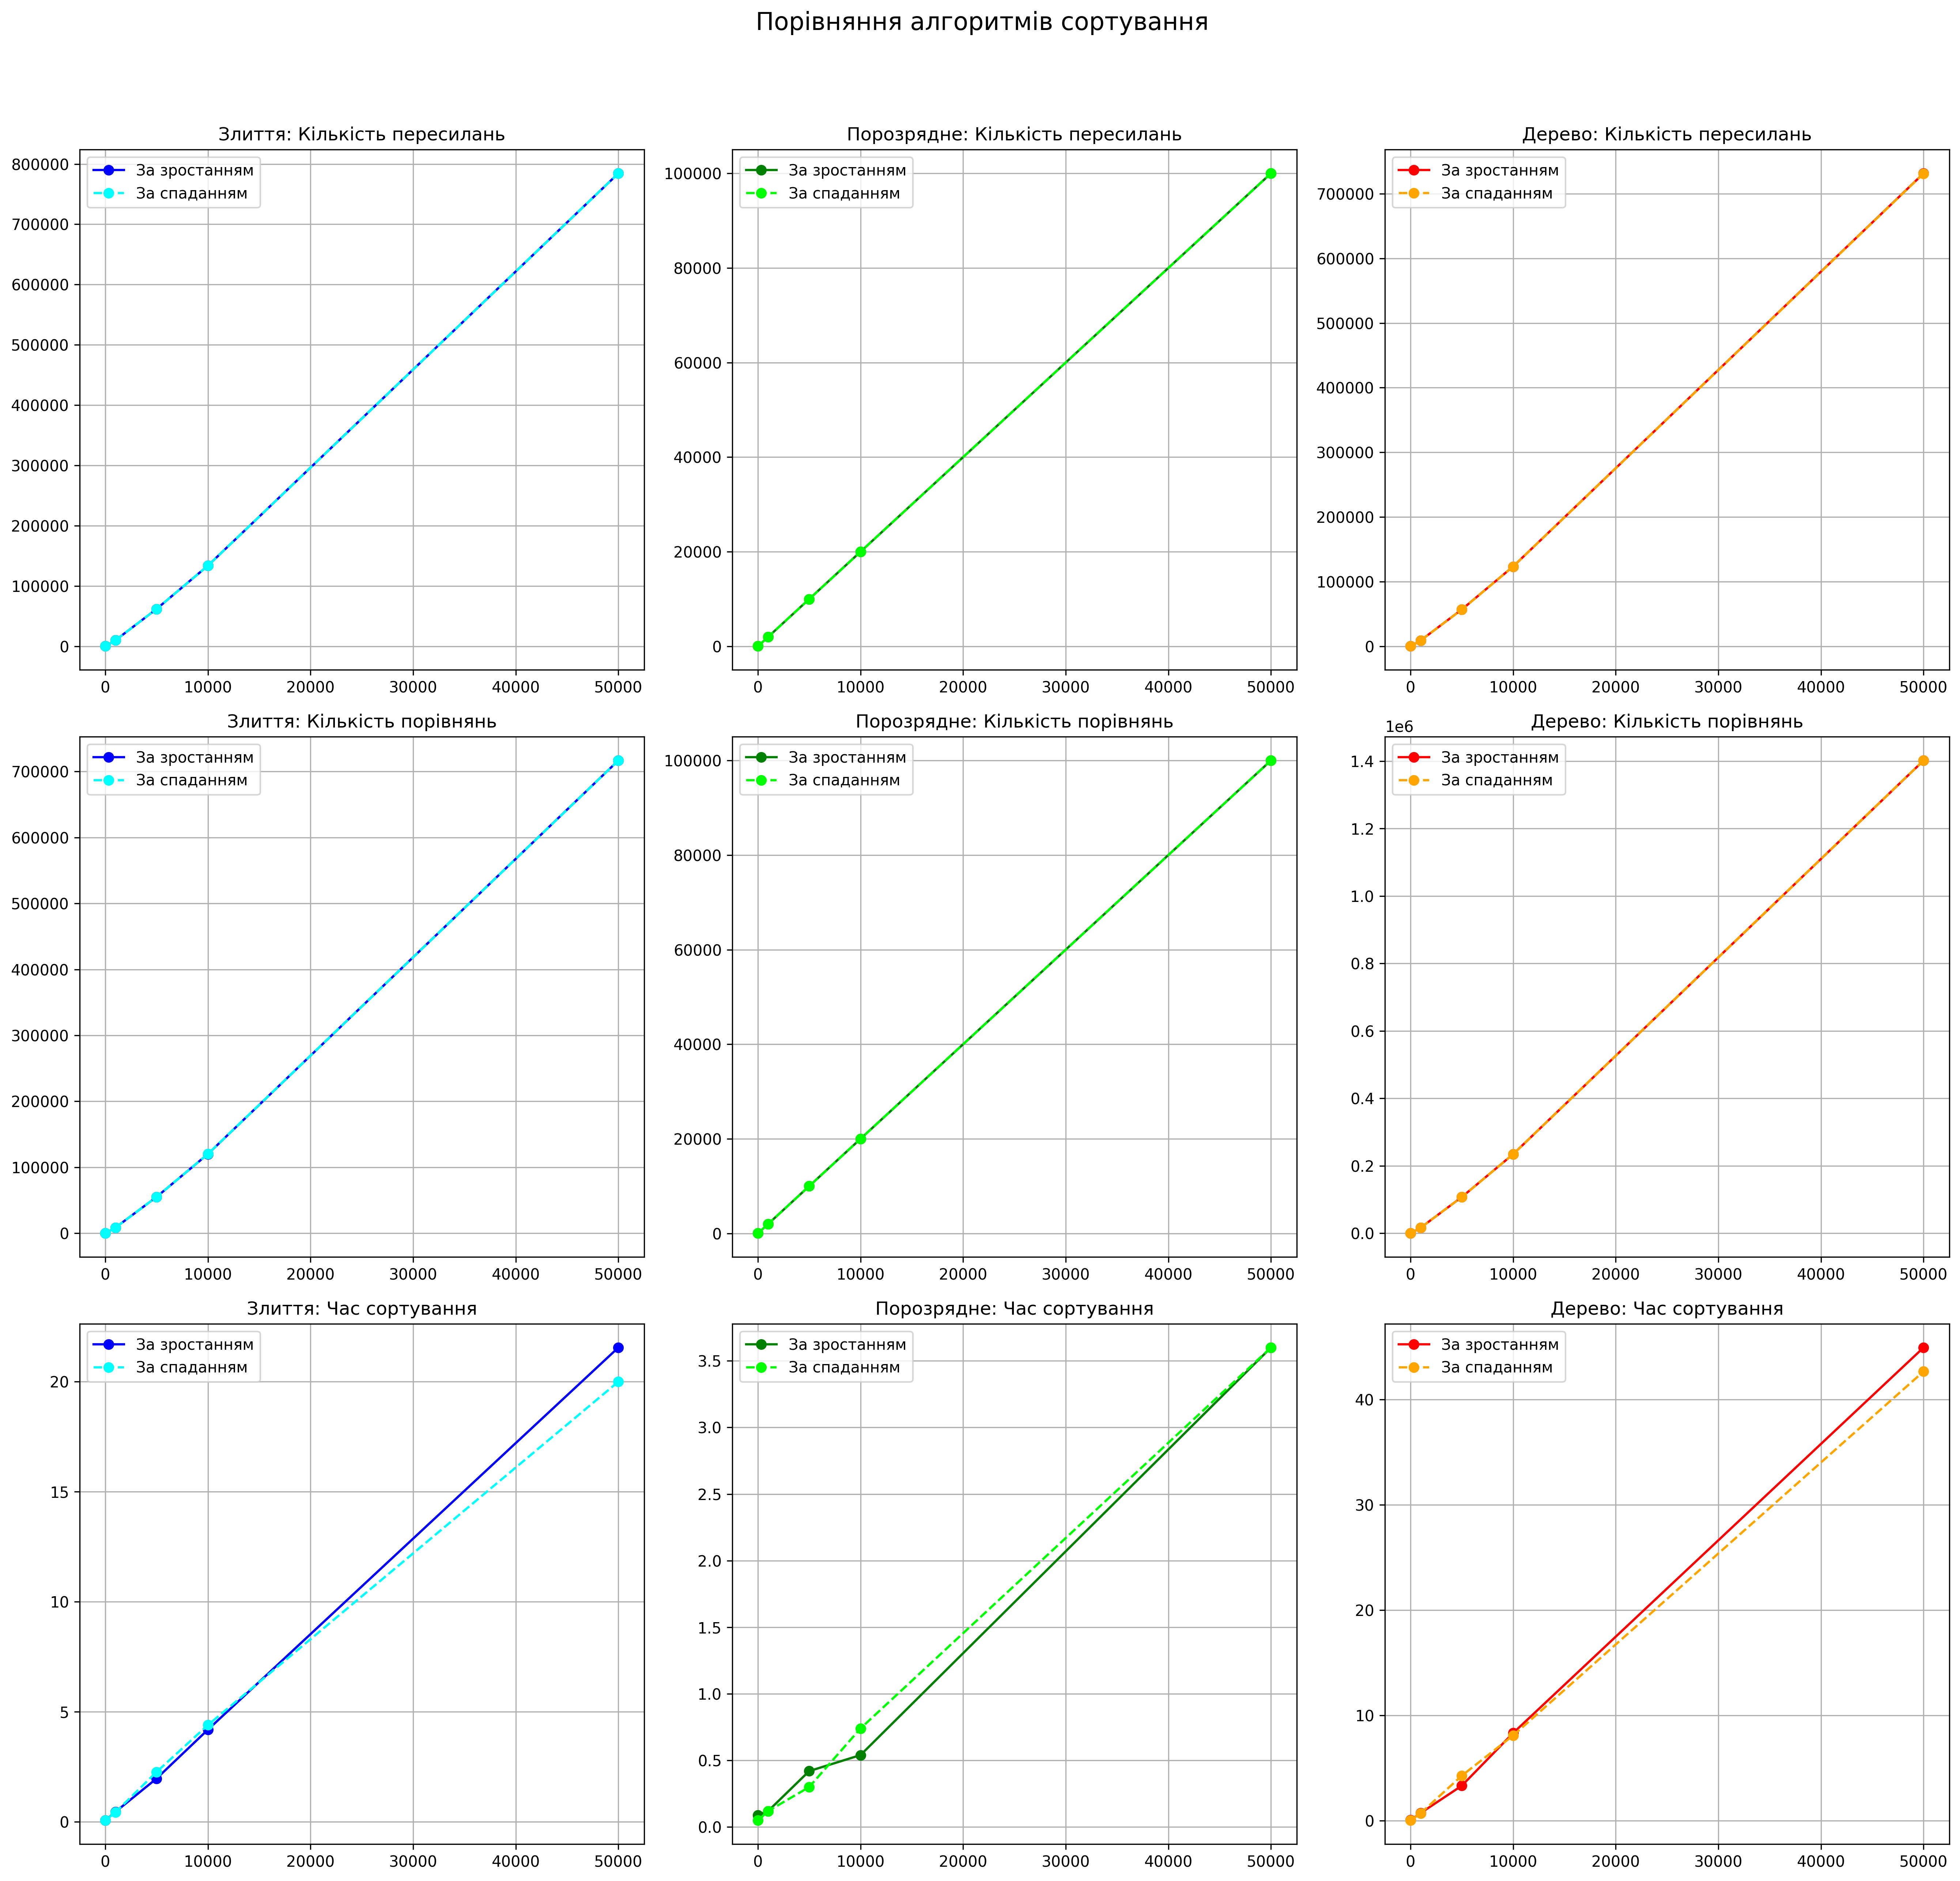
\includegraphics[width=18cm]{reports/algos/lab12/assets/plot.png}
\end{figure}

\clearpage
\section{Висновки}
В ході виконання лабораторної роботи було розроблено три алгоритми сортування відповідно варіанту завдання.\\

Після аналізу отриманих результатів для різних алгоритмів сортувань, можна зазначити що результати в залежності від зміни напрямку сортування (ask, desk) не дуже сильно змінюються для всіх сортувань.\\

Тим часом результати сортування за часом для різних напрямків сортування трішки відрізняються. Десь сортування за зростанням швидше, а десь навпаки.





